\section{One-Class Support Vector Machine}
\label{sec:OneClassSupportVectorMachine}

This algorithm is based on the kernelized \gls{svm} algorithm. While the standard application is to find the hyperplane that separates two classes, in this case the aim is to separate the instances from the origin. If a new instance is too close to the origin (of an augmented hyperspace), then it is considered an outlier. It was introduced in 2001 by M\"{u}ller \cite{mullerOneClassSVM}.

\subsection{Training}
As an example, we refere to the same dataset used in the previous sections for the \gls{dbscan} and {\gls{gmm}} algorithms. The training of the version implemented in \texttt{sklearn} require to specify the kernel to use, and the parameter $\nu$ that is the upper bound on the fraction of outlier. Training the algorithm on the dataset, with Gaussian kernel and $\nu=0.002$, we obtain the result shown in \autoref{fig:OneClassSupportVectorMachine}. 

\begin{figure}
    \centering
    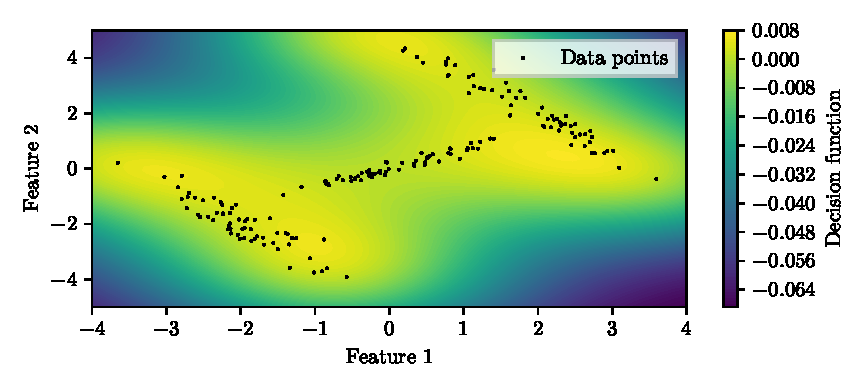
\includegraphics{images/nuSVM/Figure_1.pdf}
    \caption{One-Class Support Vector Machine decision function.}
    \label{fig:OneClassSupportVectorMachine}
\end{figure}

\subsection{Evaluation of a new instance}
\label{sec:svm_eval}
The decision function is the relative distance from the separation hyperplane, if it is positive, then the instance is considered normal, if it is negative, then the instance is considered an outlier. 

This allows us to take directly the negative of this value as a metric to evaluate the novelty of a new instance (to maintain coherence with previous sections). 

Furthrmore, simirarly to the \gls{gmm} case (\autoref{sec:gaussian}), if the train dataset contains only normal instances, we have to guess a positive value for the threshold looking at the value of the metric on the training dataset, but if we have a dataset with a known fraction of outliers, we can use the fact that $\nu$ is the upper bound on the fraction of outliers to select $\nu$ correctly in the training phase, and then use a threshold of zero for the decision function. This should make at most a $\nu$ fraction of future evaluation to be considered outliers.

\subsection{Limitations of $\nu$-\gls{svm}}

The limitations are about the sensitivity to the choice of the kernel and the parameter $\nu$, making it difficult to use in a completely unsupervised manner. 

It works well in high dimensional spaces, but it is not suited for large datasets \citepage{hands-on-geron2022}{294}